\section{Perils of disregard}
\label{sec:graph-importance}

As stated in Section \ref{sec:intro}, the development of transportation demand models aims to evaluate the impact of policies on a certain
transportation demand related outcome. As an example, consider the proposals from the following fictitious scenarios:
\begin{itemize}
 \item Based on input from the public, the Department of Transportation (DOT) of  is considering implementing a new parking policy.
 This proposed policy would put in place pricing changes and parking restrictions that would discourage individuals from parking in the central business district.
 The DOT (and its constituents) believes that this policy would encourage people to use more active transportation modes (e.g: walking, biking, etc..).
 \item A certain DOT is considering constructing a streetcar (trolley, tram) line in a low/mid-income area in its jurisdiction.
 Citing examples from other cities and countries, the DOT claims that the new streetcar line will create more transit oriented developments and increase economic activity in the areas surrounding the proposed project.
 \end{itemize}

%% TODO: Present an example or two of real life project proposals?

Thinking more closely about these proposals, it is clear that they assume a causal relationship between the proposed project/policy and the desired goals.
The DOT in question analyzed data, concluding that such a policy or project would cause the desired output and achieve the desired goal.
In the presented scenarios, the DOT claims that implementing the new parking policy will cause an increase the share of
active transportation modes in the central business district and that constructing the proposed streetcar line will
cause more transit oriented developments and economic activity.

Policymakers base their analyses and conclusions on hypotheses or beliefs of how the world operates.
In other words, the data analysis is based on a certain belief about the data generating process.
However, policymakers often do not present their beliefs about such data generating process.
As a result, these proposals maintain an obscure representation of how the policy or project will achieve their desired goals.

DAGs allow one to clearly encode their assumptions about the data generating process and the problem at hand.
Researchers and practitioners have made use of DAGs in fields ranging from medicine and epidemiology (\citet{shrier_platt_2008}, \citet{sung_2011}) to economics (\citet{white2011causal}) and have found them to be practical.

%% TODO: maybe insert some references of where DAGs were used?.

Likewise, as in the fields presented above, DAGs could prove useful in addressing transportation policy questions, similar to the ones presented above.
\citet{brathwaite_2018_causal} have proposed a framework illustrating how practitioners and researchers can use DAGs
 to answer such transportation modeling questions in a causal context.
However, \citet{brathwaite_2018_causal} did not show an empirical application of their framework and how it results
 in different conclusions when compared to traditional modeling approaches.

In this section, we will present an example illustrating the importance of using DAGs in transportation demand modeling efforts.
Specifically, we will illustrate how different assumptions about the data generating process result in different conclusions.
To make our point, we build upon \citet{brathwaite_2018_causal}.
Here, we present an empirical exercise using a simplified transportation modeling problem.
Before going any further, we note that this example is illustrative, and it does not reflect all complexities in a typical transportation choice modeling problem.
Indeed, it is not our primary goal in this section to recover the causal effect of the proposed intervention.
Instead, we are most interested in showing how different DAGs would result in different conclusions about the effect of the proposed intervention.

Let us assume that a company wants to reduce its workforce carbon footprint by moving its employees closer to their campus.
We would like to forecast how such an intervention would change the share of employees driving to work.
We model this travel mode choice problem based on a dataset from \citet{brathwaite_asymmetric}.
This dataset is based on the 2012 California Household Travel Survey, and it
contains approximately 4000 home-based school or work tours made by approximately 3850 individuals in the California Bay area.
The dataset includes the following eight travel modes:

\begin{itemize}
   \item Drive Alone: The individual uses a private vehicle to make the trip
   \item Shared Ride 2: The individual shares an automobile ride with one more individual
   \item Shared Ride 3+: The individual shares an automobile ride with two or more individuals
   \item Walk-Transit-Walk: The individual uses transit, walking to their transit origin and from their transit destination to the final destination
   \item Drive-Transit-Walk: The individual uses transit, driving to access transit and walking from a transit stop to their final destination
   \item Walk-Transit-Drive: The individual uses transit, walking to access transit and driving from a transit stop to their final destination
   \item Bike: The individual uses a bike to make the trip
   \item Walk: The individual walks to make the trip
\end{itemize}

Readers interested in a more detailed description of the dataset can refer to \citet{brathwaite_asymmetric}.
For purposes of this exercise, we consider the Multinomial Logit model defined in \citet{brathwaite_asymmetric} as the true outcome generating process.

The systematic utility equations of the adopted multinomial logit model are specified as follows:
\begin{align*}
\textrm{Utility} \left(\textrm{Drive Alone}\right) &= \beta_{\textrm{travel\_time}} \times \textrm{Travel\_Time} + \beta_{\textrm{cost\_per\_distance\_drive_alone}} \times \textrm{Cost\_per\_Distance}\left(\textrm{da}\right) \\
    &\quad + \beta_{\textrm{autos}} \times \textrm{Number\_of\_Autos} \\
\textrm{Utility} \left(\textrm{Shared Ride 2}\right) &= ASC_{\textrm{shared\_ride\_2}} + \beta_{\textrm{time\_drive}} \times \textrm{Travel\_Time} \\
    &\quad + \beta_{\textrm{cost\_per\_distance\_shared\_ride\_2}} \times \textrm{Cost\_per\_Distance}_{ \textrm{sr2} } + \beta_{\textrm{autos}}  \times \textrm{Number\_of\_Autos} \\
    &\quad + \beta_{\textrm{cross\_bay}} \times \textrm{Cross\_Bay} + \beta_{\textrm{hh\_size}} \times \textrm{HH\_Size} \\
    &\quad + \beta_{\textrm{n\_kids\_hh}} \times \textrm{Number\_of\_kids} \\
\textrm{Utility} \left(\textrm{Shared Ride 3+}\right) &= ASC_{\textrm{sr3+}} + \beta_{\textrm{time\_drive}} \times \textrm{Travel\_Time} \\
    &\quad + \beta_{\textrm{cost\_per\_distance\_sr3+}} \times \textrm{Cost\_per\_Distance}_{\textrm{sr3+}} + \beta_{\textrm{autos}}  \times \textrm{Number\_of\_Autos} \\
    &\quad + \beta_{\textrm{cross\_bay}} \times \textrm{Cross\_Bay} + \beta_{\textrm{hh\_size}} \times \textrm{HH\_Size} \\
    &\quad + \beta_{\textrm{n\_kids\_hh}} \times \textrm{Number\_of\_kids} \\
\textrm{Utility} \left(\textrm{Walk-Transit-Walk}\right) &= ASC_{\textrm{WTW}} + \beta_{\textrm{travel\_time\_transit}} \times \textrm{Travel\_Time} \\
    &\quad + \beta_{\textrm{travel\_cost}} \times \textrm{Travel\_Cost} \\
\textrm{Utility} \left(\textrm{Drive-Transit-Walk}\right) &= ASC_{\textrm{DTW}} + \beta_{\textrm{travel\_time\_transit}} \times \textrm{Travel\_Time} \\
    &\quad + \beta_{\textrm{travel\_cost}} \times \textrm{Travel\_Cost} \\
\textrm{Utility} \left(\textrm{Walk-Tranist-Drive}\right) &= ASC_{\textrm{WTD}} + \beta_{\textrm{travel\_time\_transit}} \times \textrm{Travel\_Time} \\
    &\quad + \beta_{\textrm{travel\_cost}} \times \textrm{Travel\_Cost} \\
\textrm{Utility} \left(\textrm{Bike}\right) &= ASC_{\textrm{Bike}} + \beta_{\textrm{travel\_distance\_bike}} \times \textrm{Travel\_Distance} \\
\textrm{Utility} \left(\textrm{Walk}\right) &= ASC_{\textrm{Walk}} + \beta_{\textrm{travel\_distance\_walk}} \times \textrm{Travel\_Distance} \\
\end{align*}

For our purposes, we assume that there are no latent variables.
The variables were chosen based on the specification of the MNL model outlined by the equations above.
We can describe the variables as follows:

\begin{itemize}
  \item Total Travel Distance: is the total travel distance for individual i and mode j, for all available modes for individual i during trip t of tour l.
  \item Total Travel Cost: is the travel cost in dollars for individual i and mode j, for all available modes for individual i during trip t of tour l.
  \item Total travel time: is the travel time in minutes for individual i and mode j, for all available modes for individual i during trip t tour l.
  \item Number of Autos: is the number of automobiles owned by individual i's household.
  \item Number of Licensed Drivers: is the number of licensed drives in individual i's household.
  \item Number of Kids: is the number of kids in individual i's household.
  \item Cross-bay trip: is a binary variable indicating whether the trip t in tour l for individual i is a cross-bay trip.
\end{itemize}

Figure \ref{fig:IND_GRAPH} illustrates the DAG where all explanatory variables are independent of each other for each utility equation.
Similarly, Figure \ref{fig:DA_causal_2} through \ref{fig:BIKE_causal_2} illustrate the causal graphs with dependent explanatory variables.
Each of these graphs is based on the utility function of each mode in the multinomial logit model specified in \citet{brathwaite_asymmetric}.

\begin{figure}
   \centering
   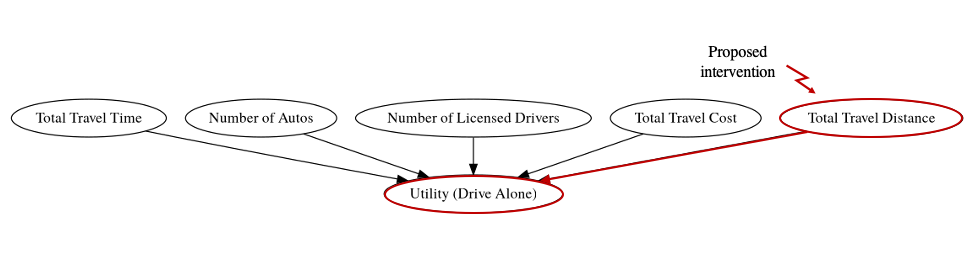
\includegraphics[width=0.5\textwidth]{Independent_graph.png}
   \caption{Causal Graph with Independent Covariates}
   \label{fig:IND_GRAPH}
\end{figure}

\begin{figure}
   \centering
   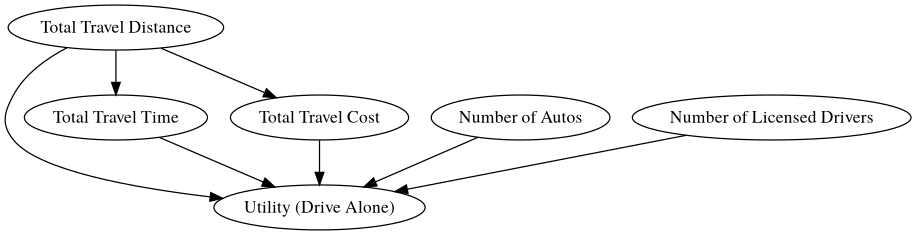
\includegraphics[width=0.5\textwidth]{DA_interacting_graph.png}
   \caption{Causal Graph for the Drive Alone Utility Function}
   \label{fig:DA_causal_2}
\end{figure}

\begin{figure}
   \centering
   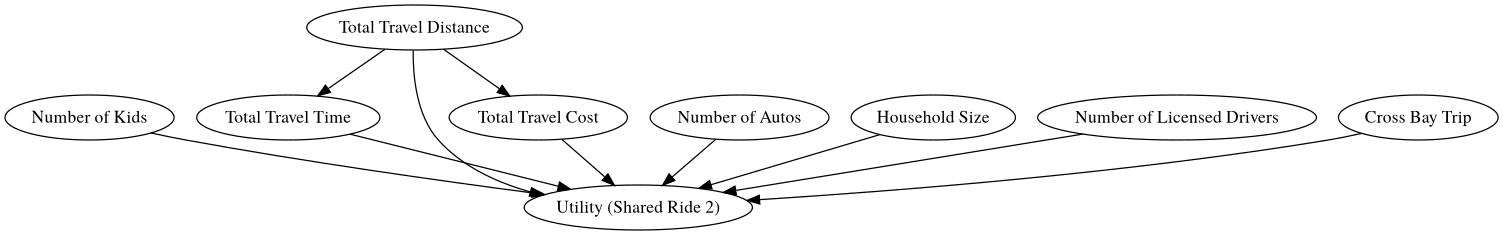
\includegraphics[width=0.5\textwidth]{SR2_interacting_graph.png}
   \caption{Causal Graph for the Shared Ride 2 Utility Function}
   \label{fig:SR2_causal_2}
\end{figure}

\begin{figure}
   \centering
   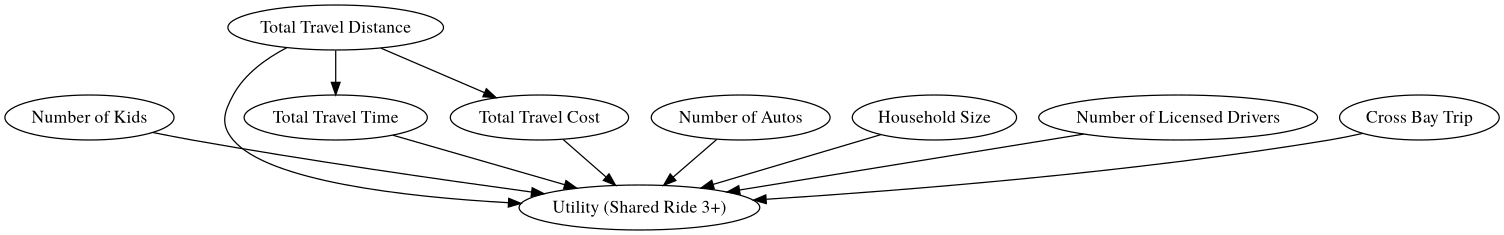
\includegraphics[width=0.5\textwidth]{SR3_interacting_graph.png}
   \caption{Causal Graph for the Shared Ride 3+ Utility Function}
   \label{fig:SR3_causal_2}
\end{figure}

\begin{figure}
   \centering
   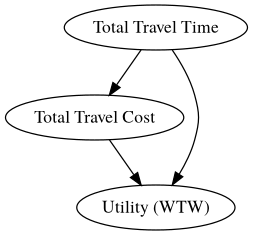
\includegraphics[width=0.5\textwidth]{WTW_interacting_graph.png}
   \caption{Causal Graph for the Walk-Transit-Walk Utility Function}
   \label{fig:WTW_causal_2}
\end{figure}

\begin{figure}
   \centering
   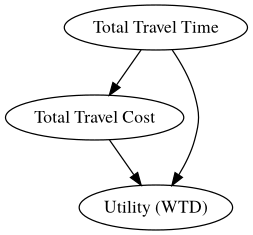
\includegraphics[width=0.5\textwidth]{WTD_interacting_graph.png}
   \caption{Causal Graph for the Walk-Transit-Drive Utility Function}
   \label{fig:WTD_causal_2}
\end{figure}

\begin{figure}
   \centering
   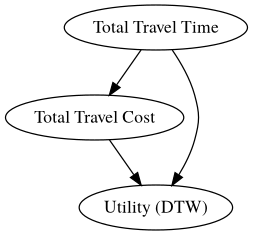
\includegraphics[width=0.5\textwidth]{DTW_interacting_graph.png}
   \caption{Causal Graph for the Drive-Transit-Walk Utility Function}
   \label{fig:DTW_causal_2}
\end{figure}

\begin{figure}
   \centering
   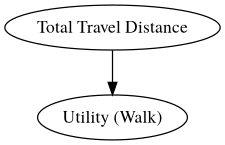
\includegraphics[width=0.5\textwidth]{WALK_interacting_graph.png}
   \caption{Causal Graph for the Shared Ride 3+ Utility Function}
   \label{fig:WALK_causal_2}
\end{figure}

\begin{figure}
   \centering
   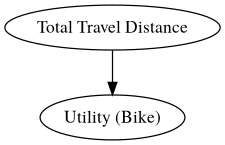
\includegraphics[width=0.5\textwidth]{BIKE_interacting_graph.png}
   \caption{Causal Graph for the Bike Utility Function}
   \label{fig:BIKE_causal_2}
\end{figure}

Using the setup described above, we conduct our simulation exercise as follows:
\begin{enumerate}

\item We build a DAG (Figure \ref{fig:IND_GRAPH}) where we assume all explanatory variables are independent of each other.
\item We simulate data based on this graph and generate outcomes based on a chosen ``true'' multinomial logit model.
\item We predict outcomes based on the mode choice model.
\item We apply the do-operator \citet{pearl_causality_2000} to our simulated data to reduce the travel distance for all individuals in the dataset. This emulates a company's decision to move its employees closer to campus.
\item We predict new outcomes based on the mode choice model.\newline
\item We build a different DAG (Figure \ref{fig:DA_causal_2} through Figure \ref{fig:BIKE_causal_2}) for each utility function based on assumptions of how explanatory variables interact and influence the outcome.
\item We use the real dataset to estimate the relationships between different variables outlined in Figure \ref{fig:DA_causal_2} through Figure \ref{fig:BIKE_causal_2}.
\item We simulate data for variables without parent nodes in Figure Figure \ref{fig:DA_causal_2} through Figure \ref{fig:BIKE_causal_2} and we use the estimated relationships from step 6 to simulate the remaining explanatory variables.
\item We then use the choice model to simulate outcome choices based on data simulated for Figure \ref{fig:DA_causal_2} through Figure \ref{fig:BIKE_causal_2}.
\item We apply the do-operator, as above, to reduce the travel distance for all individuals in the dataset and to emulate a company's decision to move its employees closer to campus.
\item We use the estimated relationships for this causal graph to simulate all the explanatory variables in Figure \ref{fig:DA_causal_2} through Figure \ref{fig:BIKE_causal_2}(namely the variables affected by travel distance).
\item We use the estimated choice model to produce outcomes based on the simulated data from the previous step.

\end{enumerate}

We repeat this simulation process several times and recover the choice probability of all modes for all individuals.
For our purposes, we focus on car-centric modes (Drive alone, Shared ride with another person,
and a shared ride with two or more individuals).
We compute the difference in mode choice probabilities from different models based on the two constructed DAGs.



We then plot histograms of the computed differences between the average probability of an individual
in our sample choosing a car centric mode before and after implementing a policy or intervention
aimed at reducing travel distance.
These differences are plotted under the two different assumptions about the data generating process illustrated in the causal graphs above.
Figure \ref{fig:histogram_probability} highlights the bias between the estimated probability of an average individual choosing a car centric mode.
This difference shows the importance of considering the data generating process when estimating transportation demand models aiming to forecast the impact of proposed policies.

\begin{figure}
   \centering
   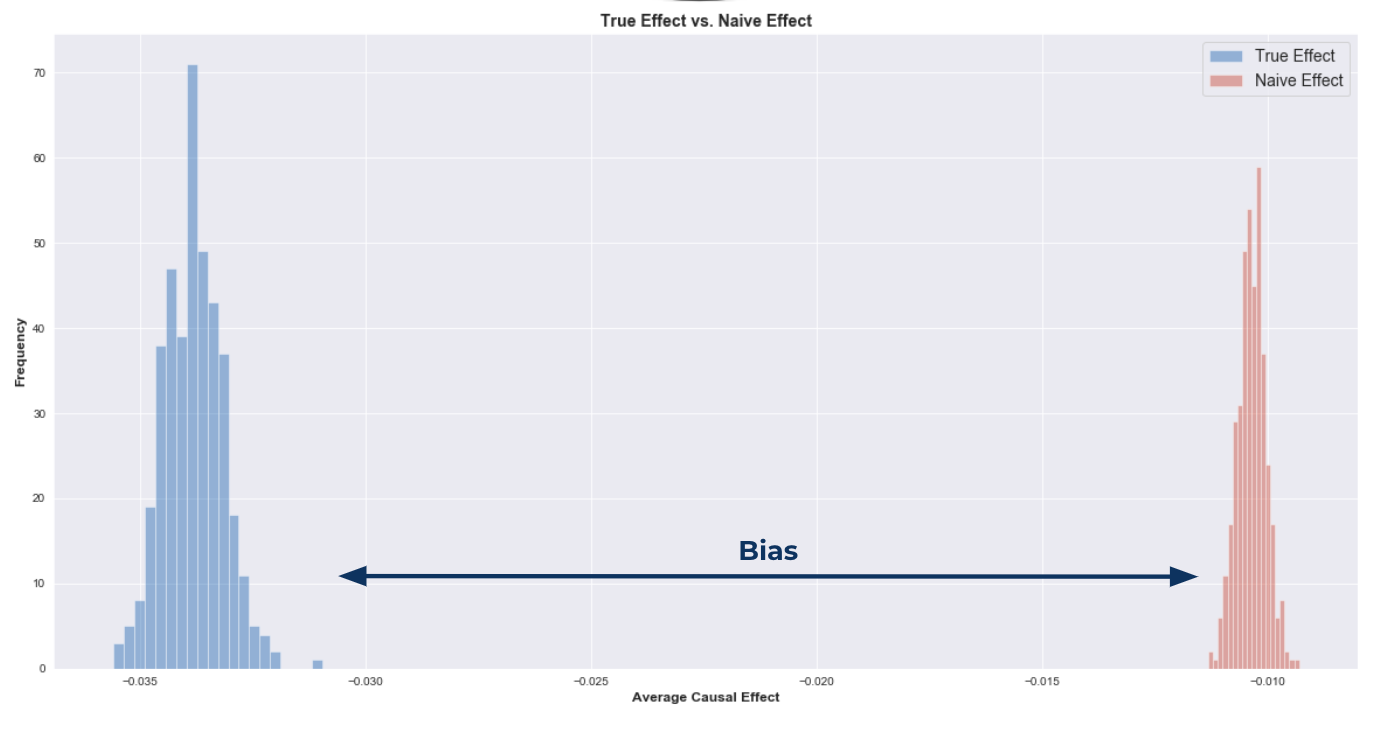
\includegraphics[width=0.5\textwidth]{histogram_selection_on_obs.png}
   \caption{Histograms of the probability of choosing Car Centric Modes under Different Data Generating processes.}
   \label{fig:histogram_probability}
\end{figure}

The data generating process might not be easily distinguishable in the majority of situations, mainly due to the complexity of the real world.
Therefore, constructing a causal graph that represents the data generating process as much as possible is not an easy task.
To prepare readers to create causal graphs, the next section will provide a brief overview of them and their history in choice modelling.
Then, Section \ref{sec:graph-construction} explores this topic and includes detailed guidance on how to build causal graphs representing the researchers beliefs about the data generating process.
Section \ref{sec:graph-testing} follows up with guidance on how to test one's causal graphs against one's data.
